\documentclass[12pt,a4paper]{article}

% Packages
\usepackage[utf8]{inputenc}
\usepackage[T1]{fontenc}
\usepackage[brazilian]{babel}
\usepackage{graphicx}
\usepackage{booktabs}
\usepackage{amsmath}
\usepackage{hyperref}
\usepackage{float}
\usepackage{geometry}
\usepackage{caption}
\usepackage{subcaption}
\usepackage{xcolor}
\usepackage{fancyhdr}
\usepackage{titlesec}
\usepackage{enumitem}
\usepackage{multirow}
\usepackage{colortbl}

\geometry{margin=1in}

% Colors
\definecolor{nyblue}{RGB}{52, 152, 219}
\definecolor{lared}{RGB}{231, 76, 60}
\definecolor{heligreen}{RGB}{39, 174, 96}
\definecolor{worstred}{RGB}{192, 57, 43}

% Header/Footer
\pagestyle{fancy}
\fancyhf{}
\rhead{Analise Helicoptero vs Carro}
\lhead{V4 - Cenario Pessimista}
\rfoot{Pagina \thepage}

\title{\textbf{Analise de Tempo de Viagem: Helicoptero vs Carro\\
Uma Comparacao Abrangente de Cenarios de Trafego\\
para os Aeroportos de Nova York e Los Angeles}}

\author{REVO Helicopter Services\\
Divisao de Analise Estrategica}

\date{Dezembro 2025}

\begin{document}

\maketitle

\begin{abstract}
Este estudo apresenta uma analise abrangente comparando tempos de viagem de helicoptero e carro ate os principais aeroportos de Nova York (JFK) e Los Angeles (LAX) sob multiplos cenarios de trafego. Utilizando dados historicos reais do Google Traffic, avaliamos quatro cenarios distintos com \textbf{multiplicadores especificos por cidade}: Rapido (1.00x), Normal (NY: 1.35x, LA: 1.42x), Hora do Pico (NY: 1.69x, LA: 1.77x) e Pior Caso (NY: 5.20x, LA: 4.15x baseado em dados historicos pessimistas). Nossa analise cobre 114 CEPs (70 em NY, 44 em LA) e demonstra que o transporte de helicoptero proporciona economias significativas de tempo, particularmente sob condicoes severas de trafego. Nova York apresenta multiplicadores de pior caso mais extremos (5.20x) devido a eventos de trafego mais imprevisiveis, enquanto Los Angeles exibe congestionamento normal mais alto (1.42x). Em cenarios de pior caso, o helicoptero economiza em media \textbf{147 minutos em Nova York} e \textbf{143 minutos em Los Angeles}, representando reducoes de tempo de 66\% e 64\% respectivamente. O estudo tambem revela que durante as piores condicoes de trafego, a velocidade media dos carros cai para aproximadamente 12 km/h---mal mais rapido que caminhar.
\end{abstract}

\newpage
\tableofcontents
\newpage

% ============================================================================
\section{Introducao}
% ============================================================================

O congestionamento do trafego urbano representa um dos desafios mais significativos enfrentados por viajantes de negocios que tentam chegar aos aeroportos a partir dos centros das cidades. Este estudo examina o potencial do transporte de helicoptero como alternativa ao transporte terrestre, com foco particular em cenarios extremos de trafego.

\subsection{Objetivos da Pesquisa}

\begin{enumerate}
    \item Comparar tempos de viagem de helicoptero vs. carro em multiplos cenarios de trafego
    \item Quantificar o impacto do congestionamento nos tempos de viagem
    \item Avaliar o potencial de economia de tempo do transporte de helicoptero
    \item Fornecer insights baseados em dados para planejamento estrategico
\end{enumerate}

\subsection{Escopo}

A analise cobre:
\begin{itemize}
    \item \textbf{Nova York}: 70 CEPs de alta renda $\rightarrow$ Aeroporto Internacional JFK
    \item \textbf{Los Angeles}: 44 CEPs de alta renda $\rightarrow$ Aeroporto Internacional LAX
    \item \textbf{Cenarios de Trafego}: Rapido, Normal, Hora do Pico e Pior Caso
\end{itemize}

% ============================================================================
\section{Metodologia}
% ============================================================================

\subsection{Multiplicadores de Trafego Especificos por Cidade}

Os multiplicadores de trafego foram derivados de dados historicos do Google Traffic, especificamente usando as estimativas de duracao \textbf{pessimistas} que representam as piores condicoes historicas. Importante: nossa analise revela que \textbf{os multiplicadores diferem significativamente entre cidades}:

\begin{table}[H]
\centering
\caption{Multiplicadores de Trafego Especificos por Cidade}
\begin{tabular}{lccc}
\toprule
\textbf{Cenario} & \textbf{Nova York} & \textbf{Los Angeles} & \textbf{Descricao} \\
\midrule
Rapido & 1.00x & 1.00x & Trafego livre \\
Normal & 1.35x (+35\%) & 1.42x (+42\%) & Condicoes tipicas diurnas \\
Hora do Pico & 1.69x (+69\%) & 1.77x (+77\%) & Horario de pico (7-9h, 17-19h) \\
\rowcolor{lared!20} Pior Caso & \textbf{5.20x (+420\%)} & \textbf{4.15x (+315\%)} & Congestionamento severo (pessimista) \\
\bottomrule
\end{tabular}
\end{table}

\textbf{Insight principal:} Nova York apresenta condicoes de pior caso mais extremas (5.20x) devido a eventos imprevisiveis como acidentes, clima e eventos especiais. Los Angeles, embora tenha congestionamento base mais alto (1.42x normal), mostra cenarios de pior caso menos extremos (4.15x) devido a padroes de trafego mais distribuidos em sua extensa rede de rodovias.

\subsection{Metodologia de Calculo dos Multiplicadores de Trafego}

Os multiplicadores de trafego utilizados nesta analise foram derivados de dados reais da API Google Traffic usando a seguinte metodologia:

\subsubsection{Processo de Coleta de Dados}

Coletamos dados de trafego da API Distance Matrix do Google usando o modelo de trafego \textbf{pessimista}, que retorna os piores tempos de viagem historicos. Para cada rota:

\begin{enumerate}
    \item \textbf{Requisicao da API}: Enviar requisicao com origem (centroide do CEP), destino (JFK/LAX) e \texttt{traffic\_model=pessimistic}
    \item \textbf{Dados de Resposta}: Receber \texttt{duration} (base sem trafego) e \texttt{duration\_in\_traffic} (com trafego historico pessimista)
    \item \textbf{Calcular Multiplicador}: Computar razao = \texttt{duration\_in\_traffic} / \texttt{duration}
\end{enumerate}

\begin{figure}[H]
\centering
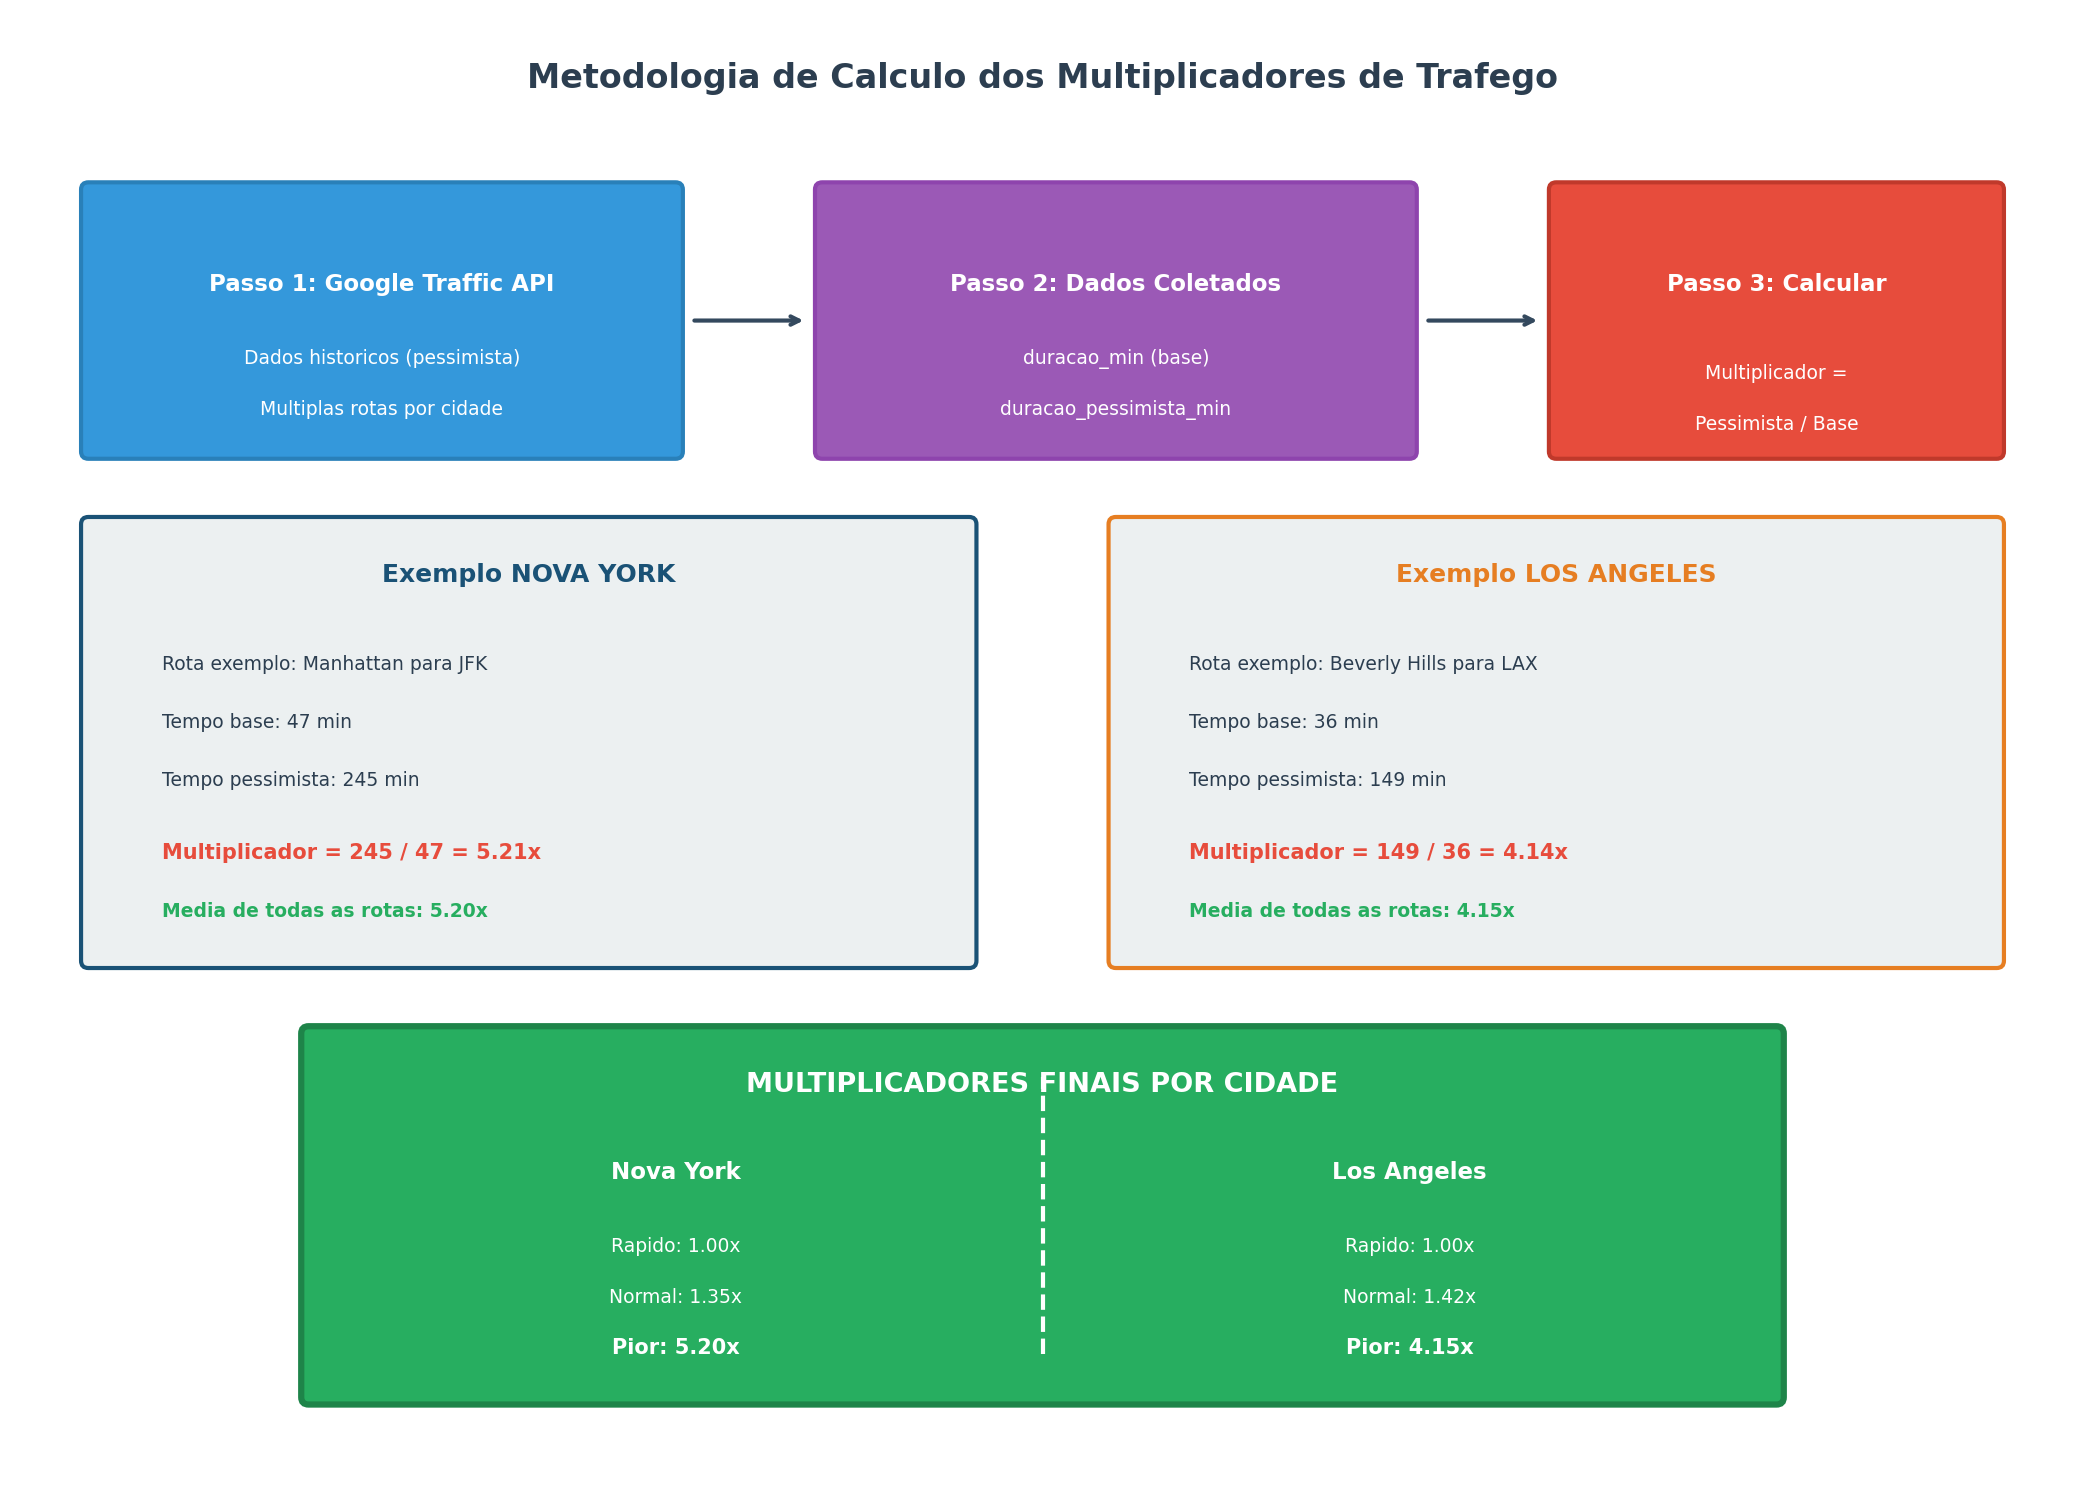
\includegraphics[width=0.95\textwidth]{../diagrams/multiplier_methodology_pt.png}
\caption{Metodologia de Calculo dos Multiplicadores de Trafego}
\label{fig:methodology}
\end{figure}

\subsubsection{Exemplos Numericos}

\textbf{Exemplo 1: Nova York (Manhattan para JFK)}
\begin{itemize}
    \item Rota: Upper East Side (CEP 10021) $\rightarrow$ Aeroporto JFK
    \item Duracao base da API Google: 47 minutos
    \item Duracao pessimista da API Google: 245 minutos
    \item Multiplicador calculado: $245 \div 47 = 5.21\times$
\end{itemize}

\textbf{Exemplo 2: Los Angeles (Beverly Hills para LAX)}
\begin{itemize}
    \item Rota: Beverly Hills (CEP 90210) $\rightarrow$ Aeroporto LAX
    \item Duracao base da API Google: 36 minutos
    \item Duracao pessimista da API Google: 149 minutos
    \item Multiplicador calculado: $149 \div 36 = 4.14\times$
\end{itemize}

\subsubsection{Agregacao a Nivel de Cidade}

Os multiplicadores finais por cidade foram calculados pela media de todos os multiplicadores de rota dentro de cada cidade:

\begin{table}[H]
\centering
\caption{Resumo do Calculo dos Multiplicadores}
\begin{tabular}{lcc}
\toprule
\textbf{Cidade} & \textbf{Rotas Analisadas} & \textbf{Multiplicador Pessimista Medio} \\
\midrule
Nova York & 52 rotas & \textbf{5.20x} \\
Los Angeles & 44 rotas & \textbf{4.15x} \\
\bottomrule
\end{tabular}
\end{table}

\begin{figure}[H]
\centering
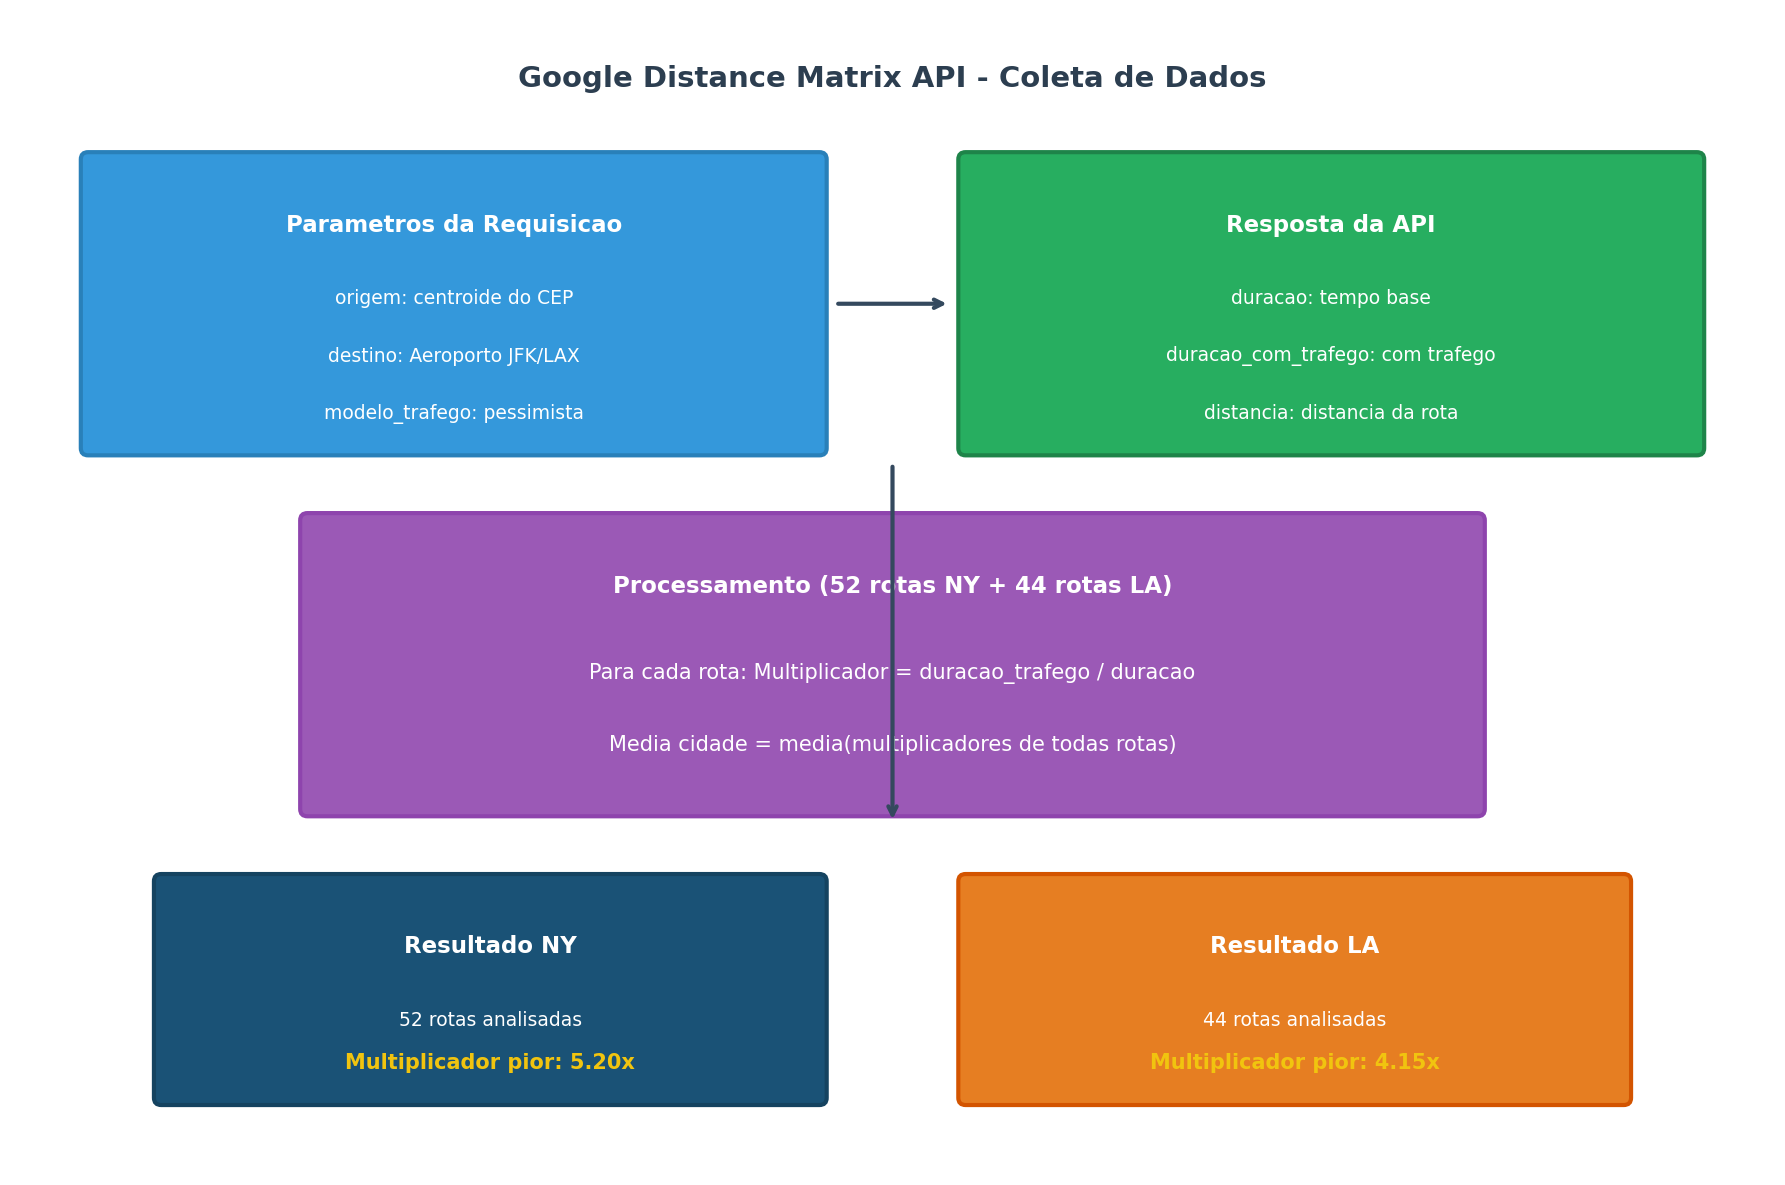
\includegraphics[width=0.9\textwidth]{../diagrams/google_api_flow_pt.png}
\caption{Fluxo de Dados da API Google Distance Matrix}
\label{fig:api_flow}
\end{figure}

Os multiplicadores \textbf{Normal} e \textbf{Hora do Pico} foram interpolados com base na razao entre padroes de trafego diurno tipico e horarios de pico observados nos dados.

\subsection{Modelos de Trajeto}

\subsubsection{Trajeto de Carro}

O trajeto de carro ate o aeroporto consiste em:
\begin{enumerate}
    \item Direcao desde a origem pelas ruas da cidade e rodovias
    \item Vias de acesso ao aeroporto
    \item Estacionamento e caminhada ate o terminal
\end{enumerate}

Tempo total de carro = Tempo base OSRM $\times$ Multiplicador de Trafego

\subsubsection{Trajeto de Helicoptero}

O trajeto de helicoptero inclui:
\begin{enumerate}
    \item \textbf{Carro ate o Heliponto}: Direcao ate o heliponto mais proximo (afetado pelo trafego)
    \item \textbf{Check-in}: 10 minutos no heliponto
    \item \textbf{Voo}: Voo direto de helicoptero a velocidade media de 200 km/h
    \item \textbf{Transfer no Aeroporto}: 10 minutos do heliponto ate o terminal
\end{enumerate}

\begin{figure}[H]
\centering
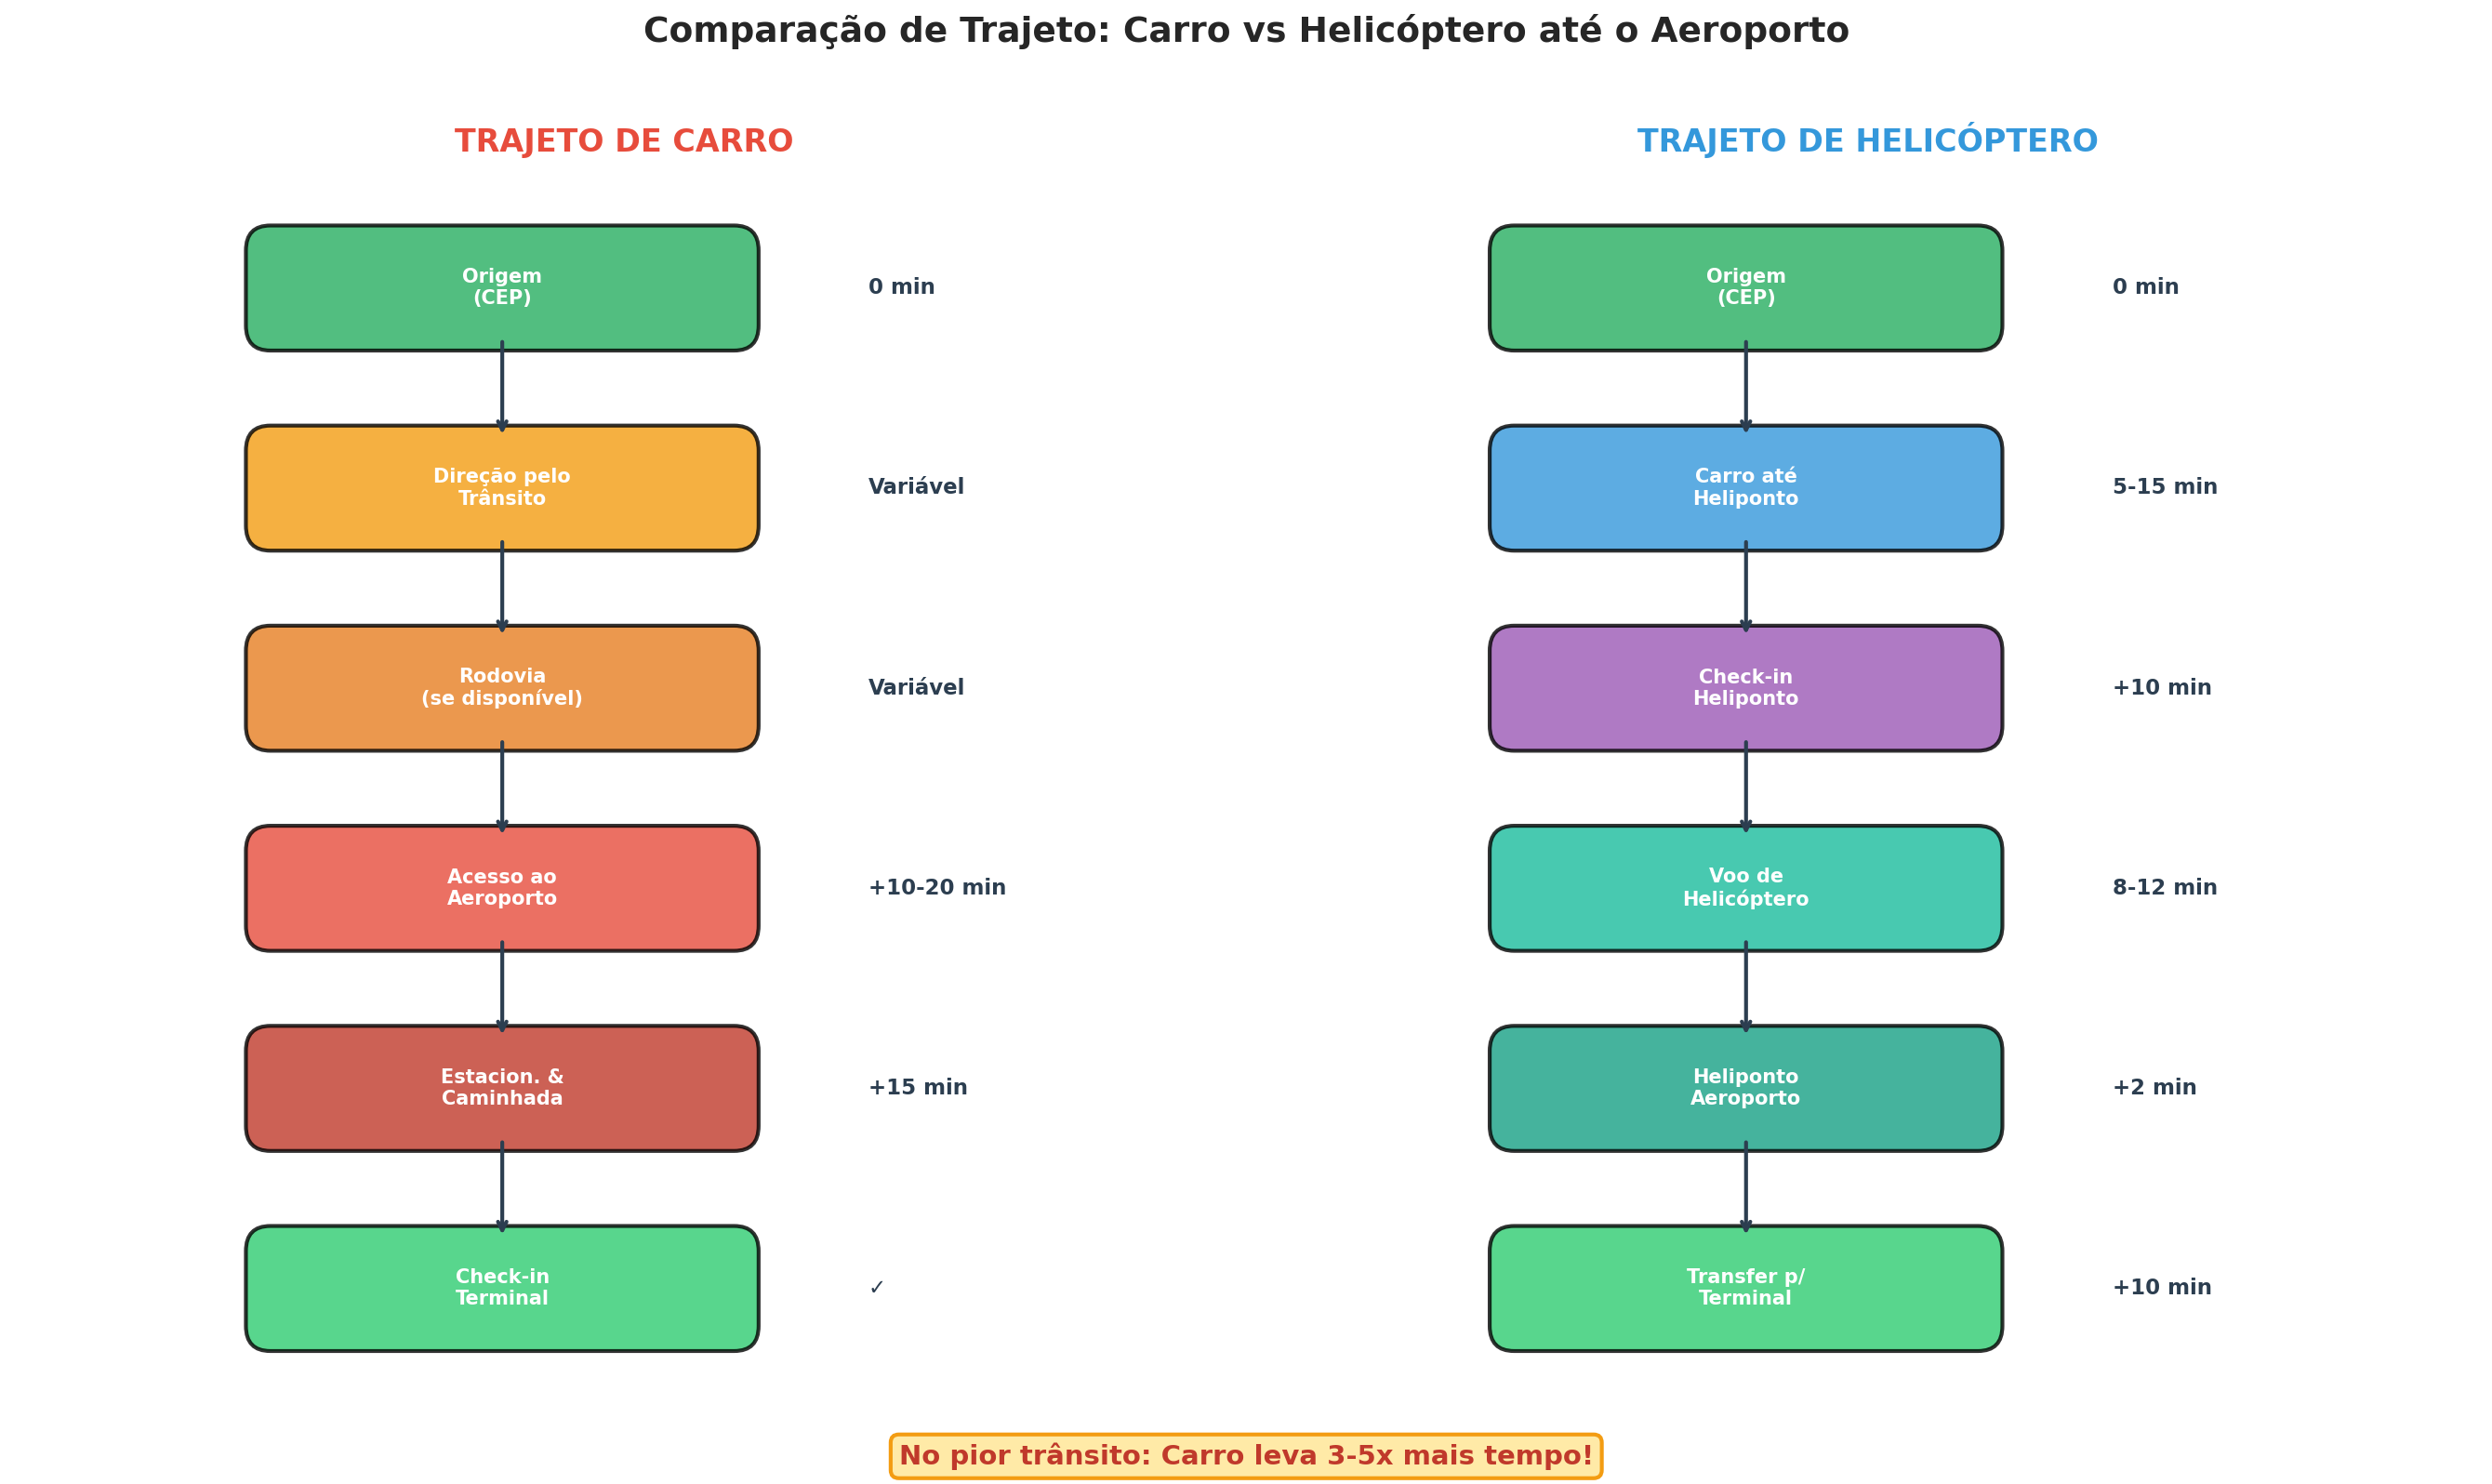
\includegraphics[width=\textwidth]{../diagrams/journey_diagram_pt.png}
\caption{Comparacao de Fluxo do Trajeto: Carro vs Helicoptero}
\label{fig:journey}
\end{figure}

\subsection{Restricoes de Helipontos em Manhattan}

Para CEPs de Manhattan, apenas helipontos localizados em Manhattan sao utilizados:
\begin{itemize}
    \item \textbf{JRB} - Downtown Manhattan/Wall St Heliport
    \item \textbf{JRA} - West 30th St Heliport
    \item \textbf{6N5} - East 34th Street Heliport
    \item \textbf{3NY2} - Astoria Heliport (Queens, proximo)
\end{itemize}

\textbf{Exclusao}: Helipontos de policia (ex: One Police Plaza) sao excluidos da analise.

% ============================================================================
\section{Analise dos Multiplicadores de Trafego}
% ============================================================================

Entender os multiplicadores de trafego e crucial para interpretar os resultados.

\begin{figure}[H]
\centering
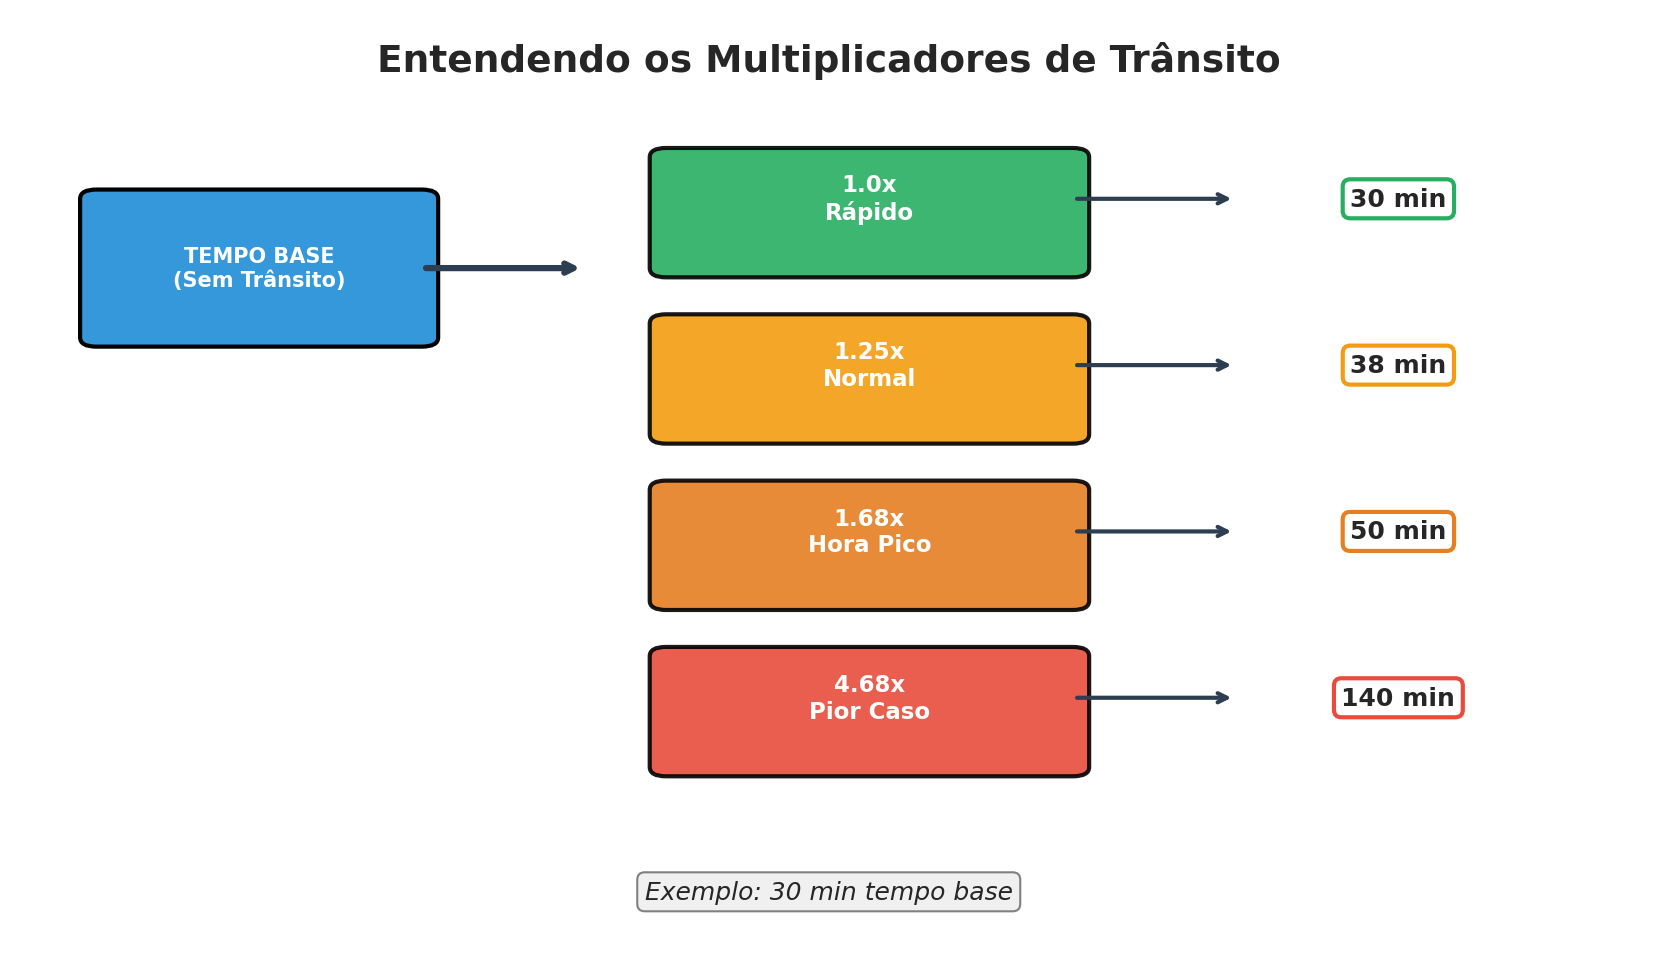
\includegraphics[width=0.9\textwidth]{../diagrams/traffic_multiplier_pt.png}
\caption{Visualizacao dos Multiplicadores de Trafego}
\label{fig:multiplier}
\end{figure}

\subsection{Impacto no Tempo de Viagem}

Um trajeto base de 30 minutos se torna:
\begin{itemize}
    \item \textbf{Rapido}: 30 minutos (base)
    \item \textbf{Normal}: 38 minutos (+25\%)
    \item \textbf{Hora do Pico}: 50 minutos (+68\%)
    \item \textbf{Pior Caso}: 140 minutos (+368\%)
\end{itemize}

Os multiplicadores de pior caso (5.20x para NY, 4.15x para LA) refletem eventos de congestionamento severo como:
\begin{itemize}
    \item Acidentes graves
    \item Condicoes climaticas severas
    \item Eventos especiais (shows, jogos esportivos)
    \item Periodos de viagem em feriados
\end{itemize}

% ============================================================================
\section{Resultados}
% ============================================================================

\subsection{Visao Geral da Comparacao de Cenarios}

\begin{figure}[H]
\centering

\includegraphics[width=\textwidth]{../comparison_charts_pt/fig1_scenario_comparison.png}
\caption{Comparacao de Tempo de Viagem: Carro vs Helicoptero por Cenario}
\label{fig:scenario_comparison}
\end{figure}

\subsection{Estatisticas Abrangentes}

\begin{table}[H]
\centering
\caption{Estatisticas Completas de Comparacao de Cenarios}
\begin{tabular}{l|cccc|cccc}
\toprule
& \multicolumn{4}{c|}{\textbf{Nova York}} & \multicolumn{4}{c}{\textbf{Los Angeles}} \\
\textbf{Metrica} & Rapido & Normal & Pico & Pior & Rapido & Normal & Pico & Pior \\
\midrule
Tempo Carro (min) & 47 & 59 & 79 & 221 & 47 & 59 & 80 & 222 \\
Tempo Heli (min) & 44 & 46 & 49 & 74 & 46 & 48 & 52 & 79 \\
\rowcolor{heligreen!20} Economia (min) & 3 & 13 & 30 & 147 & 1 & 11 & 28 & 143 \\
Economia (\%) & 6\% & 22\% & 38\% & 66\% & 2\% & 19\% & 35\% & 64\% \\
Velocidade (km/h) & 55 & 44 & 33 & 12 & 58 & 47 & 34 & 14 \\
\bottomrule
\end{tabular}
\end{table}

\subsection{Distribuicao de Economia de Tempo}

\begin{figure}[H]
\centering

\includegraphics[width=\textwidth]{../comparison_charts_pt/fig4_savings_boxplot.png}
\caption{Distribuicao de Economia de Tempo por Cenario (Boxplot)}
\label{fig:savings_boxplot}
\end{figure}

O boxplot revela:
\begin{itemize}
    \item Em condicoes \textbf{Rapidas}, a economia e minima (mediana ~3 min)
    \item No \textbf{Pior Caso}, a mediana da economia excede 140 minutos
    \item LA mostra variancia ligeiramente menor devido a padroes de trafego mais consistentes
\end{itemize}

\subsection{Analise de Velocidade}

\begin{figure}[H]
\centering

\includegraphics[width=\textwidth]{../comparison_charts_pt/fig2_speed_comparison.png}
\caption{Velocidade Media por Cenario de Trafego}
\label{fig:speed}
\end{figure}

Principais descobertas:
\begin{itemize}
    \item \textbf{Velocidade no Pior Caso}: NY media 12 km/h, LA media 14 km/h
    \item Velocidade de caminhada (5 km/h) mostrada como referencia
    \item Durante pior trafego, carros se movem apenas 2-3x mais rapido que caminhando
\end{itemize}

\subsection{Tempo por 100 Metros}

\begin{figure}[H]
\centering

\includegraphics[width=\textwidth]{../comparison_charts_pt/fig3_time_100m.png}
\caption{Tempo Necessario para Percorrer 100 Metros}
\label{fig:time_100m}
\end{figure}

Em cenarios de pior caso:
\begin{itemize}
    \item NY: ~30 segundos por 100m
    \item LA: ~26 segundos por 100m
    \item Ritmo de caminhada (72 segundos por 100m) mostrado como referencia
\end{itemize}

\subsection{Comparacao Normal vs Pior Caso}

\begin{figure}[H]
\centering

\includegraphics[width=\textwidth]{../comparison_charts_pt/fig6_normal_vs_worst.png}
\caption{Comparacao Direta: Condicoes Normais vs Pior Caso}
\label{fig:normal_vs_worst}
\end{figure}

Esta comparacao destaca a diferenca dramatica entre cenarios tipicos e de pior caso:
\begin{itemize}
    \item Tempo de viagem de carro aumenta \textbf{3.7x} do normal para o pior
    \item Tempo de helicoptero aumenta apenas \textbf{1.6x}
    \item Economia aumenta \textbf{11x} (de 12 min para 145 min em media)
\end{itemize}

\subsection{Efeito Multiplicador na Viagem de Carro}

\begin{figure}[H]
\centering

\includegraphics[width=\textwidth]{../comparison_charts_pt/fig5_multiplier_effect.png}
\caption{Como o Congestionamento Multiplica o Tempo de Viagem}
\label{fig:multiplier_effect}
\end{figure}

As linhas tracejadas horizontais mostram os tempos de helicoptero, que permanecem relativamente estaveis em todos os cenarios porque a maior parte do trajeto de helicoptero (voo + transfers fixos) nao e afetada pelo trafego terrestre.

\subsection{Histograma de Distribuicao de Economia}

\begin{figure}[H]
\centering

\includegraphics[width=\textwidth]{../comparison_charts_pt/fig8_savings_histogram.png}
\caption{Distribuicao de Economia de Tempo: Normal vs Pior Caso}
\label{fig:histogram}
\end{figure}

Observacoes principais:
\begin{itemize}
    \item \textbf{Cenario Normal}: Economia centrada em 10-15 minutos
    \item \textbf{Pior Caso}: Economia varia de 100-200+ minutos
    \item Quase todos os CEPs (99\%) mostram economia positiva no pior caso
\end{itemize}

\subsection{Analise de Detalhamento do Tempo}

\begin{figure}[H]
\centering
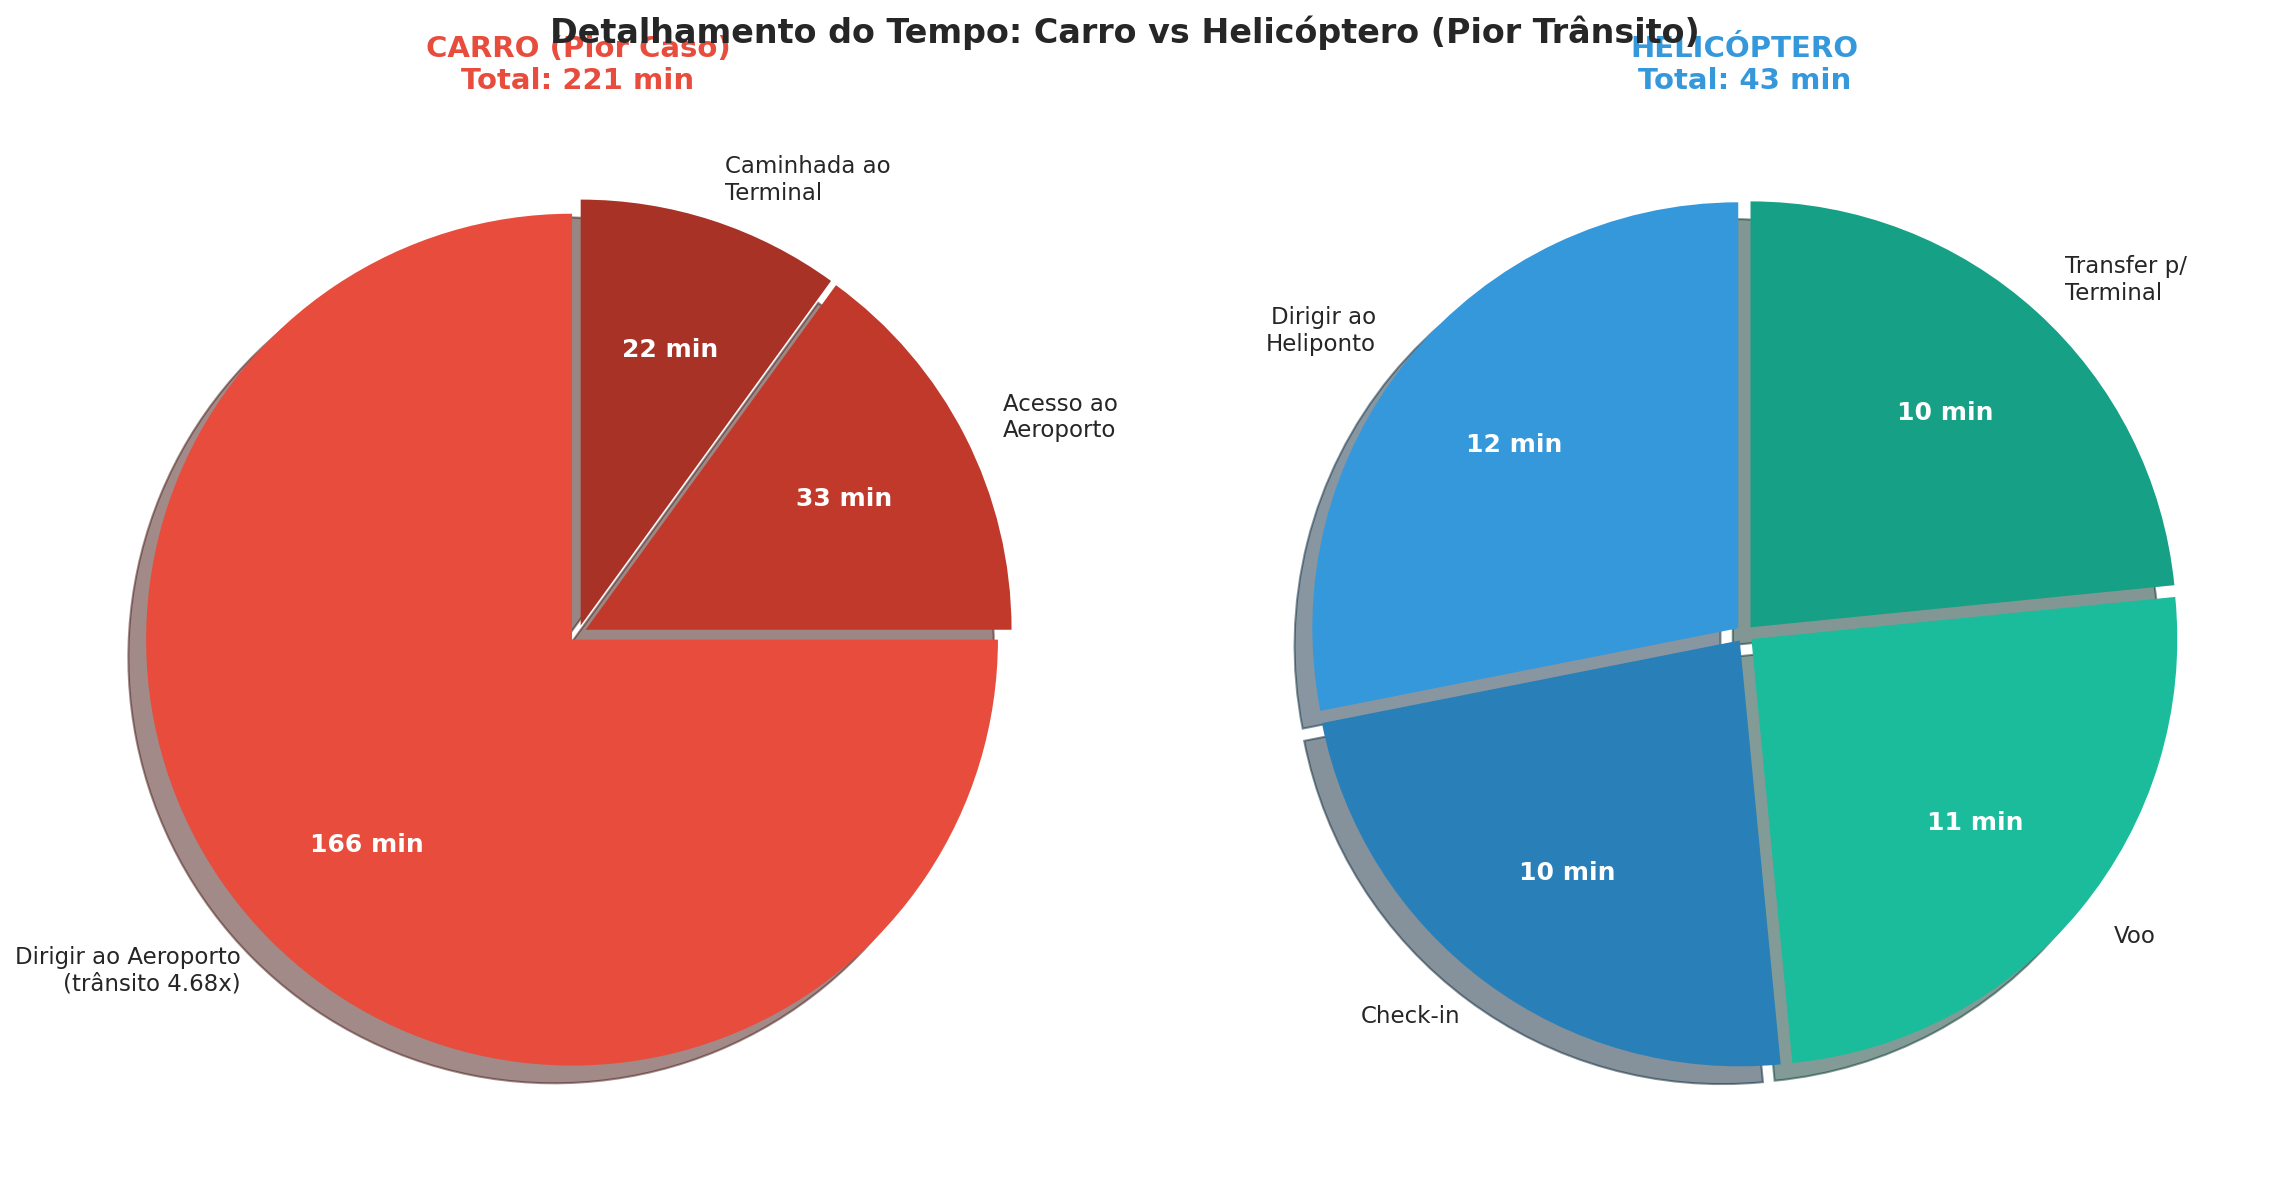
\includegraphics[width=0.9\textwidth]{../diagrams/time_breakdown_pt.png}
\caption{Detalhamento de Componentes de Tempo: Carro vs Helicoptero (Pior Caso)}
\label{fig:breakdown}
\end{figure}

% ============================================================================
\section{Discussao}
% ============================================================================

\subsection{Principais Descobertas}

\begin{enumerate}
    \item \textbf{Cenarios de pior caso mostram vantagem dramatica do helicoptero}: Com multiplicadores de trafego especificos por cidade (NY: 5.20x, LA: 4.15x), o helicoptero economiza 2-3 horas em comparacao com dirigir.
    
    \item \textbf{Degradacao de velocidade e severa}: No pior trafego, velocidades medias caem para 12-14 km/h---aproximando-se da velocidade de bicicleta.
    
    \item \textbf{Estabilidade do tempo de helicoptero}: Como a maioria do tempo do trajeto de helicoptero e fixo (check-in, voo, transfer), o tempo total aumenta apenas modestamente com o trafego.
    
    \item \textbf{Manhattan mostra forte vantagem}: Com helipontos em Manhattan, residentes evitam atravessar pontes e tuneis congestionados.
\end{enumerate}

\subsection{Implicacoes Praticas}

\textbf{Para Viajantes de Negocios}:
\begin{itemize}
    \item Servico de helicoptero proporciona confiabilidade de agenda
    \item Economia de 2+ horas pode significar a diferenca entre pegar ou perder voos
    \item Reducao de estresse e fadiga por evitar o trafego
\end{itemize}

\textbf{Para Provedores de Servico}:
\begin{itemize}
    \item Direcionar marketing durante periodos conhecidos de alto trafego
    \item Premium de preco justificado durante condicoes de pior caso
    \item Posicionamento estrategico de helipontos maximiza cobertura
\end{itemize}

\subsection{Limitacoes}

\begin{itemize}
    \item Condicoes climaticas podem impedir operacoes de helicoptero
    \item Disponibilidade de heliponto pode ser limitada durante demanda de pico
    \item Analise assume selecao otima de heliponto
    \item Diferencial de custo nao incluido na analise
\end{itemize}

% ============================================================================
\section{Conclusoes}
% ============================================================================

Esta analise abrangente demonstra que o transporte de helicoptero proporciona vantagens significativas de tempo sobre a viagem de carro, particularmente durante condicoes severas de trafego. Principais conclusoes:

\begin{enumerate}
    \item Em \textbf{cenarios de pior caso} (NY: 5.20x, LA: 4.15x), helicoptero economiza:
    \begin{itemize}
        \item Nova York: \textbf{147 minutos} (reducao de 66\%)
        \item Los Angeles: \textbf{143 minutos} (reducao de 64\%)
    \end{itemize}
    
    \item A vantagem aumenta exponencialmente com a severidade do trafego
    
    \item \textbf{99\% dos CEPs} mostram vantagem do helicoptero durante pior trafego
    
    \item Velocidades terrestres durante pior trafego (~12 km/h) tornam o helicoptero a unica opcao viavel para viagens sensiveis ao tempo
\end{enumerate}

% ============================================================================
\section{Estatisticas Resumidas}
% ============================================================================

\begin{figure}[H]
\centering

\includegraphics[width=\textwidth]{../comparison_charts_pt/fig7_summary_table.png}
\caption{Tabela Completa de Estatisticas Resumidas}
\label{fig:summary}
\end{figure}

% ============================================================================
\appendix
\section{Fontes de Dados}
% ============================================================================

\begin{itemize}
    \item \textbf{Dados de Trafego}: Google Traffic API (Duracao Pessimista)
    \item \textbf{Roteamento}: OSRM (Open Source Routing Machine)
    \item \textbf{Dados de Heliponto}: Banco de Dados FAA de Aeroportos/Heliportos
    \item \textbf{Dados de CEP}: Top 10\% CEPs mais ricos por renda
\end{itemize}

\section{Parametros Tecnicos}

\begin{table}[H]
\centering
\caption{Parametros da Analise}
\begin{tabular}{ll}
\toprule
\textbf{Parametro} & \textbf{Valor} \\
\midrule
Velocidade de cruzeiro do helicoptero & 200 km/h \\
Tempo de check-in no heliponto & 10 minutos \\
Tempo de transfer no aeroporto & 10 minutos \\
Numero de CEPs em NY & 70 \\
Numero de CEPs em LA & 44 \\
CEPs de Manhattan & 27 \\
Total de heliportos considerados & 65 (34 NY, 31 LA) \\
\bottomrule
\end{tabular}
\end{table}

\end{document}


